% !TEX root = ./main.tex

\section{Results}
\label{sec:results}

We report results on the Synthea dataset described in Section~\ref{sec:system}. After outlier removal, 21{,}995 of the 22{,}284 patients were used to fit the clustering model, and the remaining patients were kept as the separate group with label $-1$.

\subsection{Clustering}

To select a configuration we ran a benchmark over 63 feature subsets and several hyperparameter values, and we ranked the runs with a combined score that gives the most weight to the Gower silhouette. Table~\ref{tab:clusters} lists the best configuration for each number of clusters.

\begin{table}[t]
\caption{Best clustering configuration per number of clusters. The final pick is $k=4$.}
\label{tab:clusters}
\centering
\small
\begin{tabular}{@{}lccccc@{}}
\toprule
Config & $k$ & $\gamma$ & Silhouette & Gower & Davies-Bouldin \\
\midrule
\textbf{Final ($k{=}4$)} & \textbf{4} & auto & 0.132 & \textbf{0.350} & 2.51 \\
Best $k{=}5$ & 5 & 0.17 & 0.095 & 0.356 & 3.11 \\
Best $k{=}6$ & 6 & 0.17 & 0.029 & 0.313 & 2.59 \\
\bottomrule
\end{tabular}
\end{table}

We chose $k=4$. The five-cluster run has a slightly higher Gower silhouette (0.356 against 0.350), but only one of its clusters clears our stability threshold of about $0.20$, while in the four-cluster run all clusters do, with per-cluster values of $0.423$, $0.199$, $0.320$ and $0.396$. Since the clusters are later used as scopes for sequence mining, we prefer the smallest $k$ for which every cluster stays cohesive. The strongest features are the number of active conditions ($\eta^2 = 0.74$) and age ($\eta^2 = 0.66$) on the numerical side, and condition burden (Cramer's V $= 0.80$), gender ($0.70$), diabetes ($0.69$) and heart disease ($0.66$) on the categorical side.

Figures~\ref{fig:heatmap},~\ref{fig:numerical} and~\ref{fig:categorical} describe the final partition. The heatmap of z-scored numerical means shows a clear morbidity gradient, from cluster~0 with younger and low-burden patients to the higher-numbered clusters with more conditions and more treatment. The numerical bars confirm that active conditions and age drive most of the separation, and the categorical panel shows how condition burden, the disease flags and gender split the four groups. Read together, the clusters correspond to four recognisable populations: young low-burden patients, women of reproductive age, hypertensive adults with polypharmacy, and a pediatric or acute group.

\begin{figure}[t]
\centering
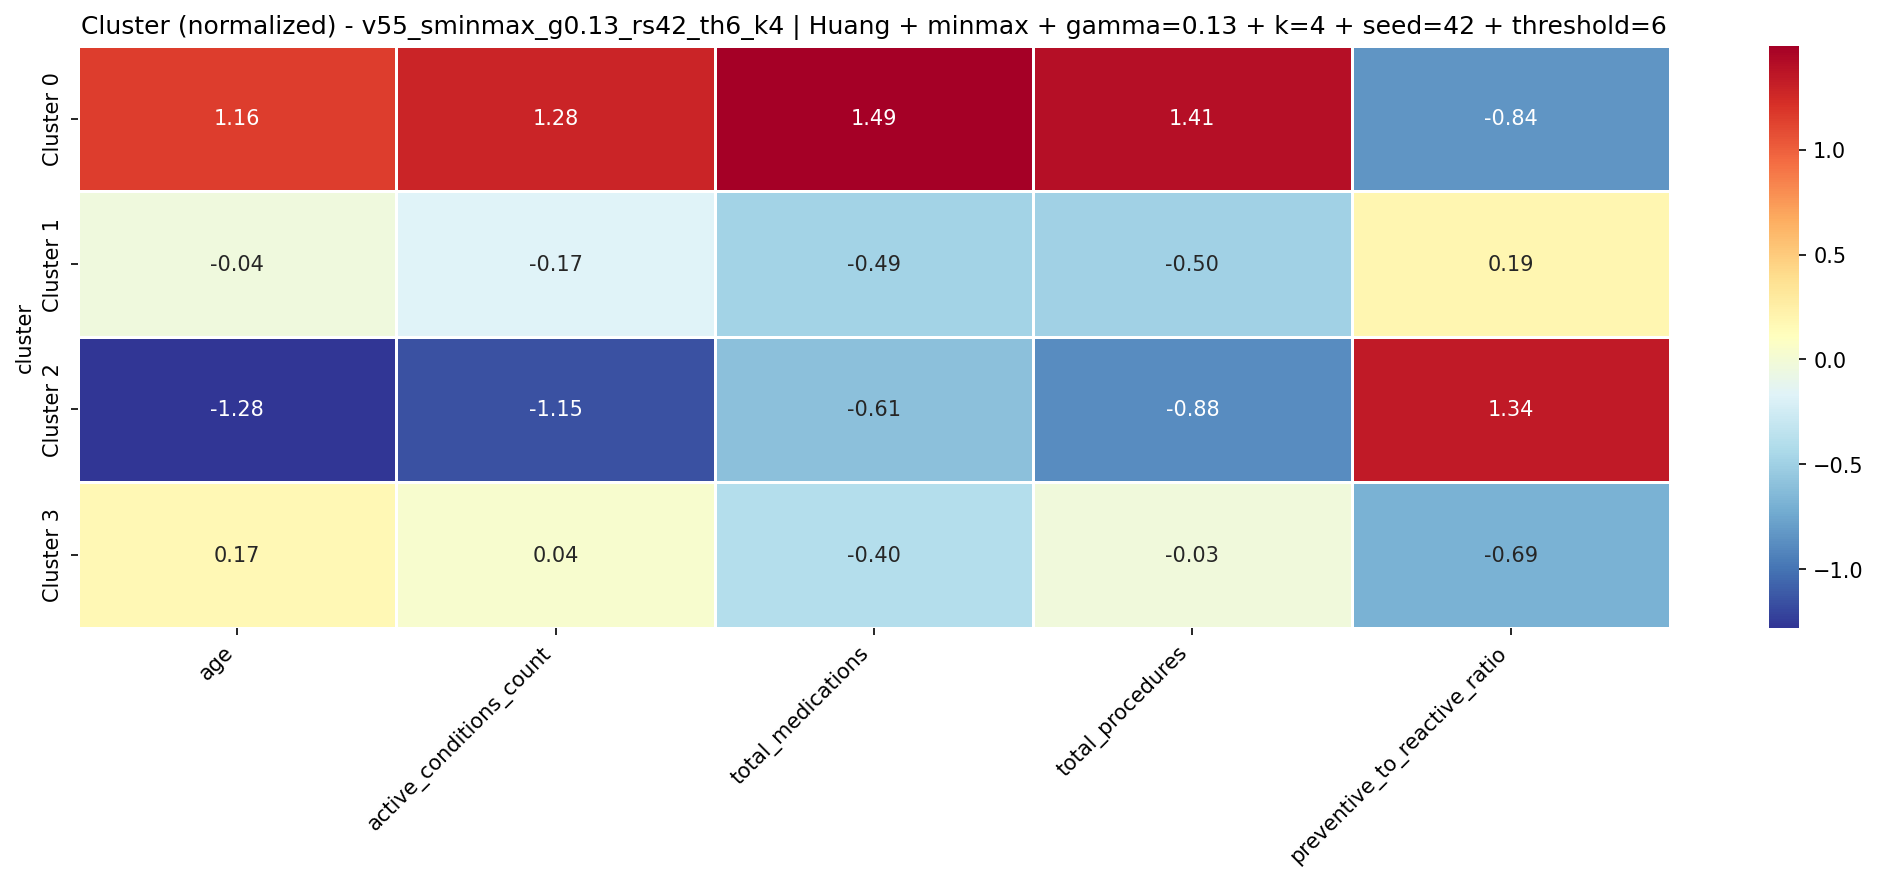
\includegraphics[width=0.92\linewidth]{figs/cluster_heatmap.png}
\caption{Z-scored numerical feature means per cluster ($k=4$). Warm colours are above the population average, cool colours below it.}
\label{fig:heatmap}
\end{figure}

\begin{figure}[t]
\centering
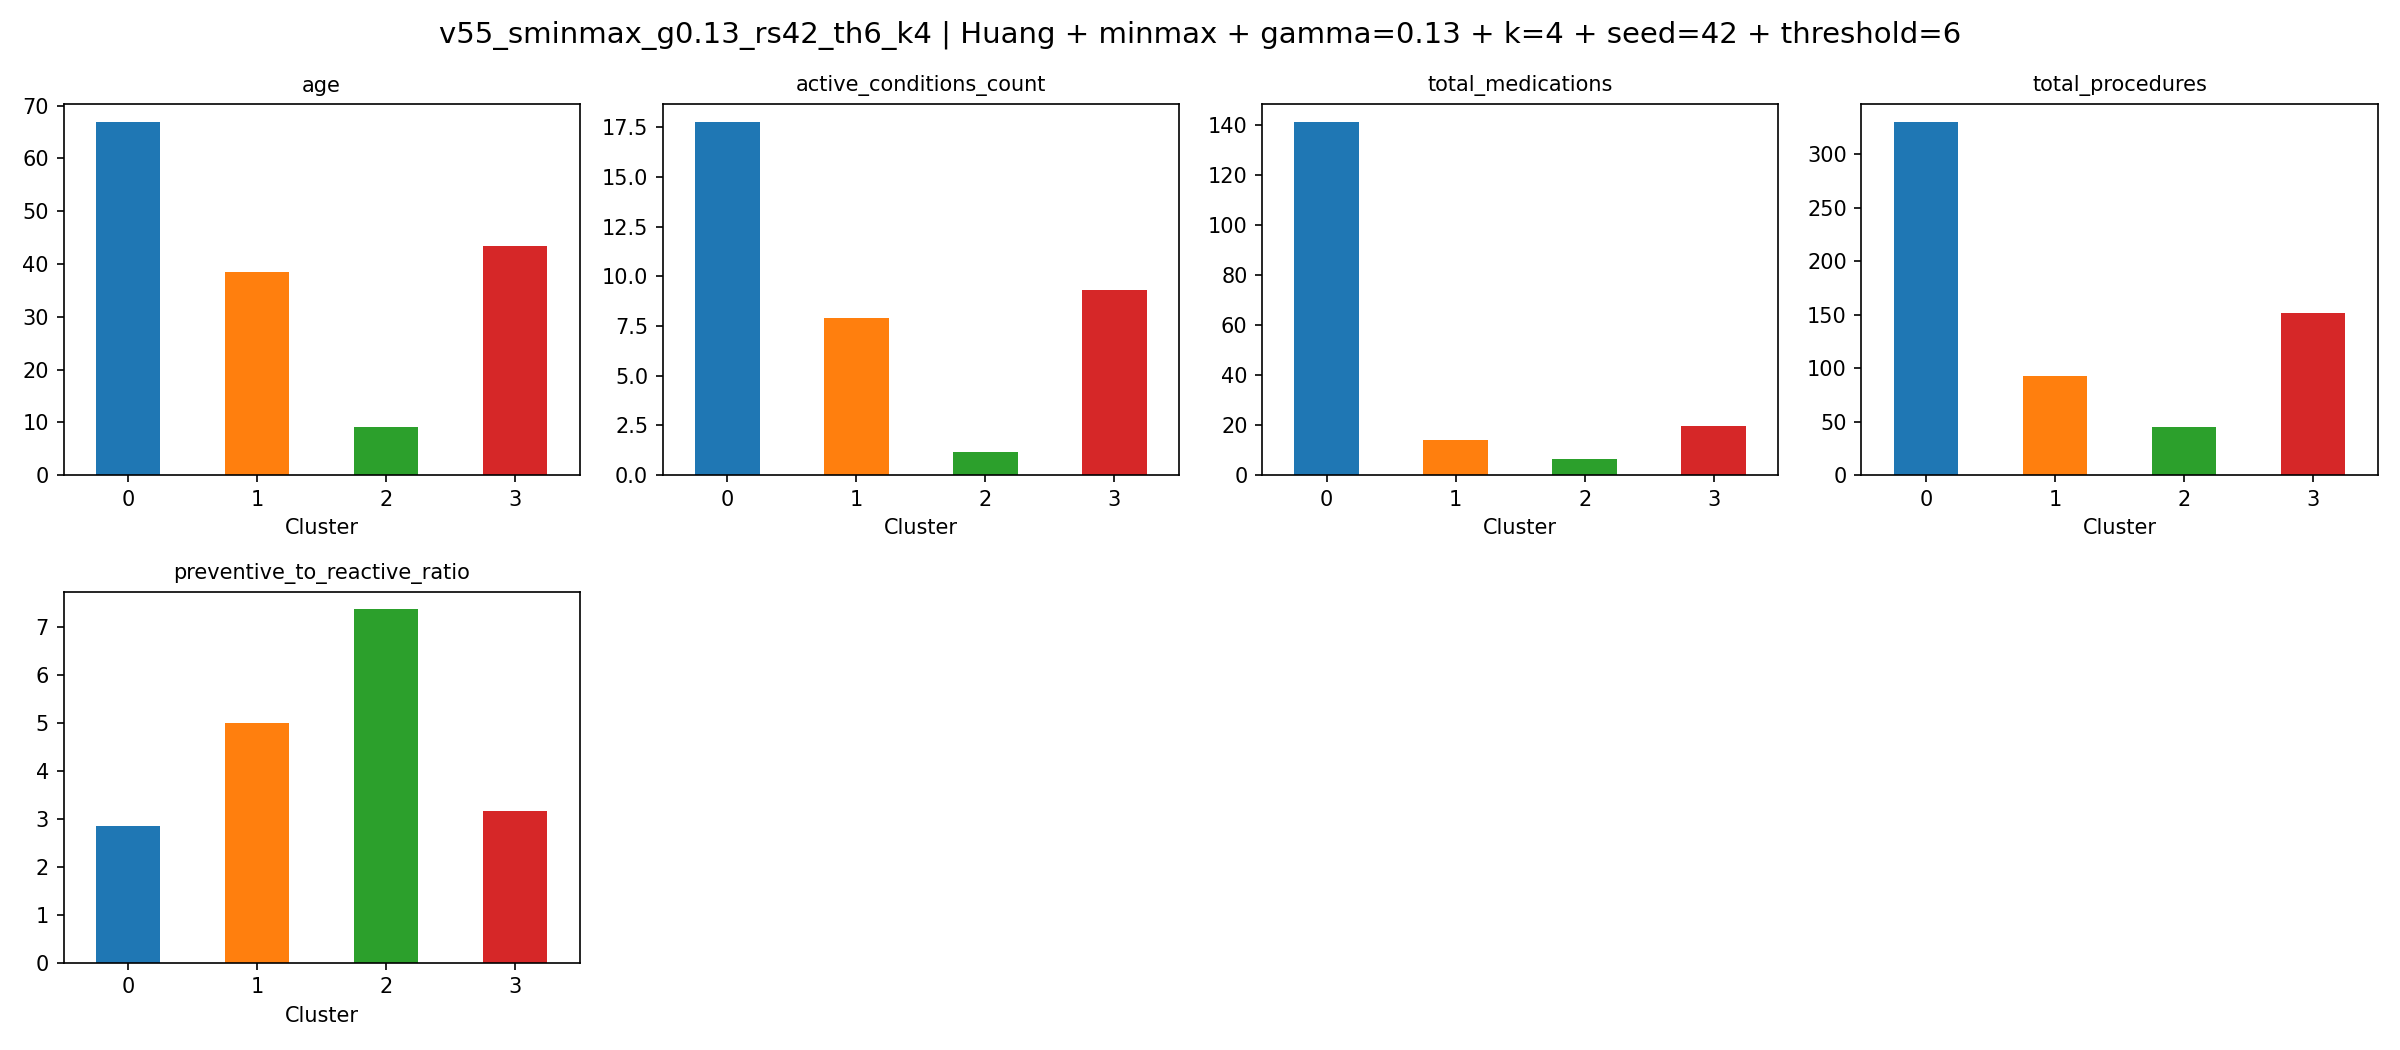
\includegraphics[width=0.92\linewidth]{figs/cluster_numerical.png}
\caption{Per-cluster means of the five numerical features.}
\label{fig:numerical}
\end{figure}

\begin{figure}[t]
\centering
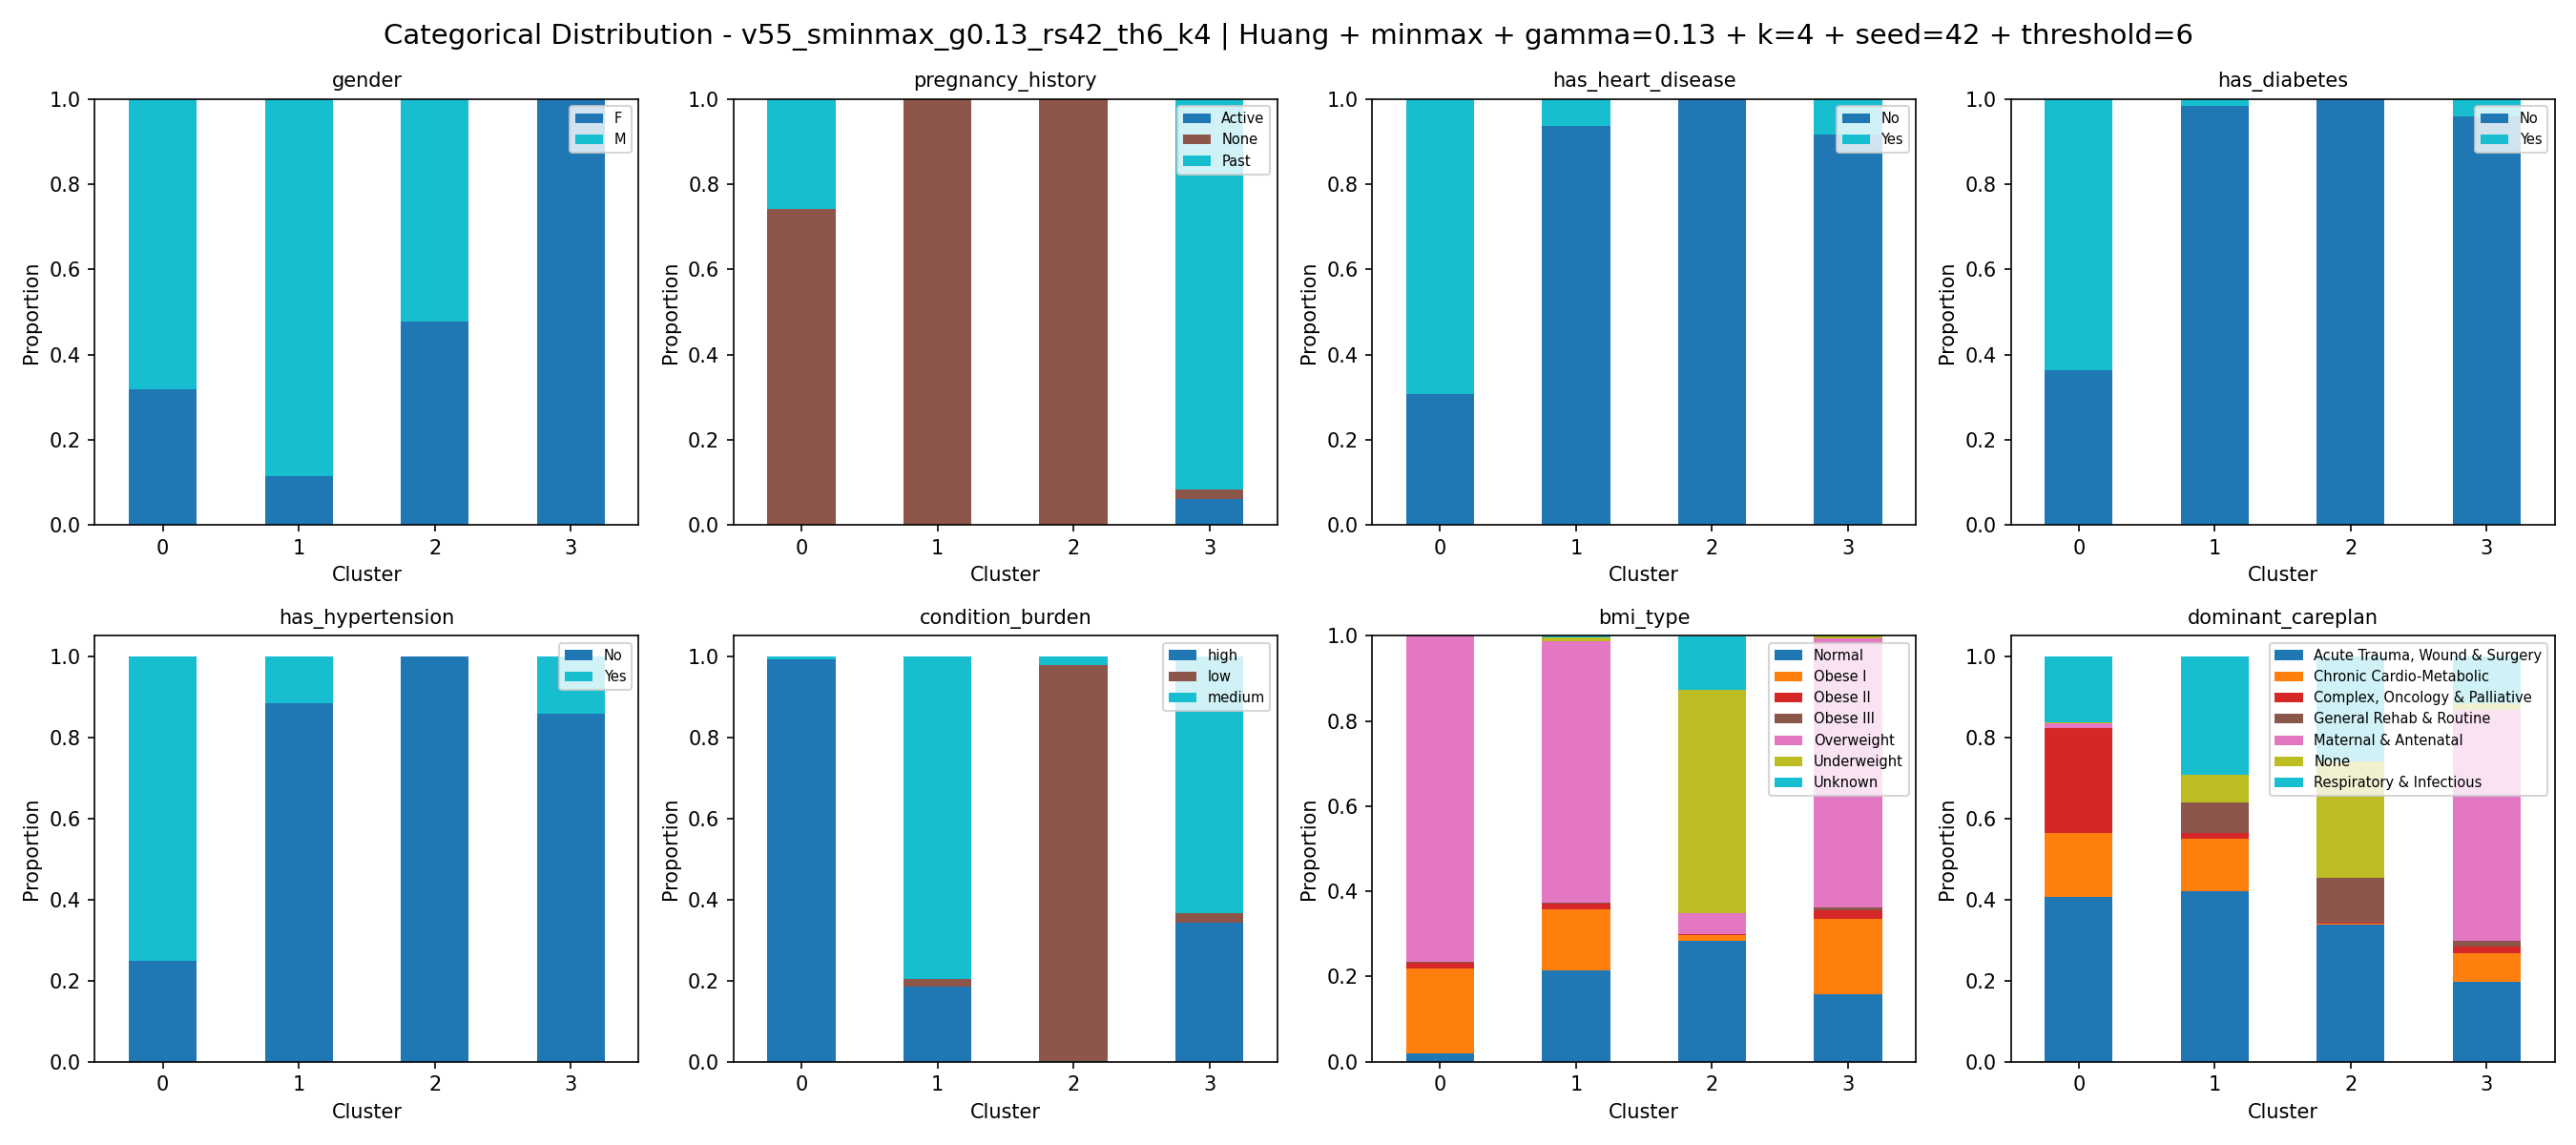
\includegraphics[width=0.92\linewidth]{figs/cluster_categorical.png}
\caption{Per-cluster proportions of the eight categorical features.}
\label{fig:categorical}
\end{figure}

\subsection{Sequence Mining}

The clearest way to show the effect of the pipeline is to compare the first and the last version of the miner on the same data. Table~\ref{tab:ablation} shows the top pattern in each case. When we rank by raw support (version v0), the best result is an administrative loop, and almost the entire top of the list is filled with near-identical dental cleaning steps that around 93\% of patients receive. After we add the GML score and the diversity selection (version v6), the top of the list becomes a set of short, clinically coherent care paths.

\begin{table}[t]
\caption{Effect of the ranking. Top pattern when ranking by support (v0) and by geometric mean lift with diversity selection (v6).}
\label{tab:ablation}
\centering
\small
\begin{tabular}{@{}p{0.08\linewidth}p{0.82\linewidth}@{}}
\toprule
Ver. & Top-ranked pattern \\
\midrule
v0 & Medication review due $\rightarrow$ Medication reconciliation $\rightarrow$ Medication review due \emph{(support 96\%, no clinical value)} \\[2pt]
v6 & Laceration $\rightarrow$ Wound care $\rightarrow$ Suture open wound \emph{(GML 0.97)} \\
\bottomrule
\end{tabular}
\end{table}

Mining each scope on its own produces between 175 and 252 frequent patterns. Table~\ref{tab:patterns} gives representative patterns from the hypertensive cluster and from the outlier scope. The hypertensive cluster is dominated by chronic-disease management, for example a furosemide and oxygen sequence for fluid overload, a dialysis and epoetin loop, and an antihypertensive drug paired with screening procedures. The outlier scope is the most striking result. Because we mine the label $-1$ group separately, high-cost pathways become visible: chemotherapy with cisplatin followed by hospice care, kidney transplantation with tacrolimus, and a recurring heart-failure sequence. These pathways are below the global support floor and would be invisible if we mined the whole cohort at once.

\begin{table}[t]
\caption{Representative mined pathways from two scopes (ranked by GML).}
\label{tab:patterns}
\centering
\small
\begin{tabular}{@{}p{0.16\linewidth}p{0.66\linewidth}r@{}}
\toprule
Scope & Pattern & GML \\
\midrule
Cluster 2 & Furosemide $\rightarrow$ Oxygen by mask $\rightarrow$ Prone position $\rightarrow$ Furosemide & 0.89 \\
Cluster 2 & Epoetin Alfa $\rightarrow$ Renal dialysis $\rightarrow$ Epoetin Alfa & 0.81 \\
Cluster 2 & Lisinopril $\rightarrow$ Depression screening $\rightarrow$ Substance-use assessment & 0.41 \\
Outliers ($-1$) & Chemotherapy + radiation $\rightarrow$ Cisplatin $\rightarrow$ Hospice care & 0.85 \\
Outliers ($-1$) & Renal review $\rightarrow$ Tacrolimus $\rightarrow$ Kidney transplantation & 0.90 \\
\bottomrule
\end{tabular}
\end{table}

Taken together, the results show that the four-cluster partition is not only defensible by its metrics but also meaningful in content. Each cluster's top patterns describe a clearly different care population, which is exactly the property we need for cluster-scoped analysis in the dashboard.
